%02/10 - Luis del Peso
\chapter{Alineamiento de secuencias por pares}
El alineamiento de secuencias es la herramienta más fundamental de la bioinformática. Permite identificar secuencias relacionadas con una secuencia dada. Como veremos, el parentesco suele implicar que las secuencias pueden tener funciones comunes y esa es una de las principales aplicaciones del alineamiento de secuencias, inferir la función de una secuencia biológica.

\section{Alineamiento de secuencias}
La alineación de secuencias es el procedimiento de ordenar dos (alineación por pares) o varias (alineación de secuencias múltiples, MSA) secuencias intentando colocar el mayor número posible de residuos idénticos o similares en el mismo registro vertical (misma columna). Los residuos no idénticos pueden colocarse en la misma columna como una falta de coincidencia o frente a un hueco en la otra secuencia. El objetivo de la alineación es maximizar el número de coincidencias (residuos idénticos o similares en la misma columna) y minimizar el número de desajustes y huecos.

\begin{figure}[htbp]
\centering
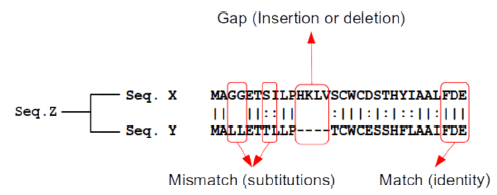
\includegraphics[width = 0.7\textwidth]{figs/pairwise-alignment.png}
\caption{\textbf{Alineamiento por pares.} La alineación por pares modela la evolución de las dos secuencias a partir de un ancestro común. En un intento de colocar los residuos derivados de la misma posición ancestral en el registro vertical, el proceso de alienación maximiza las coincidencias y minimiza las diferencias debidas a mutación de la secuencia ancestral (desajustes y lagunas). En la representación, dos residuos iguales se muestran conectados por una línea vertical. En caso de discordancia, si a nivel biológico los residuos tienen una función similar, se denota con dos puntos, mientras que si la función es diferente, se deja en blanco, al igual que en el caso de inserciones y deleciones.}
\end{figure}

¿Por qué alineamos las secuencias de este modo? En la alineación de secuencias, el supuesto subyacente es que las \textbf{secuencias que se alinean proceden de un ancestro común}. Sin embargo, como consecuencia de las mutaciones acumuladas durante la evolución, las secuencias no serán idénticas. Así pues, el reto consiste en colocar los residuos que derivan de la \textbf{misma posición ancestral} en la misma columna del alineamiento. Sin embargo, sin información sobre la secuencia ancestral y su evolución, lo mejor que podemos hacer es maximizar el número de coincidencias y minimizar el número de discordancias. En las secuencias de proteínas, las sustituciones se producen cuando una mutación (mutación sin sentido o missense) en la secuencia ancestral hace que el codón de un aminoácido se cambie por el de otro. El resultado sería la alineación de dos aminoácidos no idénticos, es decir, un desajuste. Las inserciones y deleciones (normalmente abreviadas como INDEL) se producen cuando se añaden o eliminan residuos de la secuencia ancestral. Las inserciones o deleciones (incluso las de un solo carácter) se representan como huecos en el alineamiento. El número de mutaciones aumentará a medida que las dos secuencias diverjan de su ancestro común. Así, en general, el número de coincidencias disminuye con la distancia evolutiva. En general, se puede inferir que los residuos idénticos entre secuencias probablemente también estén presentes en el ancestro. En el caso de las sustituciones y deleciones/inserciones, no se puede determinar si el ancestro era de una forma u otra, es decir, si realmente se trata de un fragmento que se ha perdido (una deleción) o un fragmento que en algún momento se insertó. 

\section{Comparación de alineamientos}
A la hora de alinear dos secuencias, se pueden producir todos los alineamientos posibles y escoger aquel que tenga el mayor número de coincidencias y el menor número de discordancias o gaps. Un alineamiento óptimo sería aquel que incluya en la misma columna residuos que derivan del mismo residuo original (es decir, alinear residuos ortólogos). Normalmente, no se conoce la secuencia del ancestro o la historia evolutiva, por lo que se intenta inferir al alinear todos los residuos idénticos o similares posibles. Para establecer el grado de similitud, se puede tener en cuenta las propiedades fisicoquímicas (hidrofobicidad, carga neta a pH fisiológico, flexibilidad de la cadena lateral) y la estructura (tamaño, presencia de anillos aromáticos). Además, si se permiten los gaps en el alineamiento, la cantidad de posibles alineamientos aumenta de forma astronómica. Por tanto, para encontrar el mejor alineamiento, se necesita:
\begin{itemize}
\item Una métrica cuantitativa que representa la similitud entre residuos.
\item Un método de puntuación que produce un valor que resume lo buena que es la alineación teniendo en cuenta todas las posiciones y huecos.
\item Un procedimiento capaz de producir todos los alineamientos posibles y puntuarlos eficazmente (y no evaluando todos los posibles alineamientos).
\end{itemize}

\subsection{Matrices de sustitución}
Como ya se ha dicho, el alineamiento consiste en reunir residuos idénticos o similares. Identificar los residuos idénticos es sencillo. Sin embargo, ¿qué entendemos por residuos similares? En el caso de los ácidos nucleicos, la función de un determinado nucleótido (su patrón de emparejamiento de bases) no suele poder sustituirse por ninguno de los demás nucleótidos. Por lo tanto, durante la alineación de secuencias de nucleótidos (normalmente) sólo nos preocupamos por las identidades \footnote{De hecho, dado que las transiciones (es decir, las sustituciones entre las purinas A y G o entre las pirimidinas C y T) son más frecuentes que las transversiones (sustituciones entre purina y pirimidina o viceversa), existen algunos esquemas de puntuación específicos para la alineación de residuos de nucleótidos no idénticos.}. Cualquier otro emparejamiento es un desajuste igualmente perjudicial. Sin embargo, en el caso de las secuencias de aminoácidos, ciertas sustituciones de aminoácidos tienen poco impacto, mientras que otras pueden abolir por completo la función/estructura de la proteína. Así, en el curso de la evolución, los residuos importantes para la función de la molécula tienden a permanecer inalterados o a ser sustituidos por un residuo similar, manteniendo así la estructura y/o la función. Por estas razones, algunas sustituciones particulares se encuentran comúnmente en proteínas relacionadas de diferentes especies. Así, para los alineamientos de proteínas asignamos una puntuación a cada par o aminoácidos que representa la probabilidad de observar la sustitución de uno por otro. Una tabla que contiene las puntuaciones de todos los posibles pares de residuos se denomina \textbf{matriz de sustitución}. Las puntuaciones de cada celda de una matriz de sustitución reflejan la probabilidad de que los dos residuos estén alineados porque son verdaderos homólogos en comparación con la probabilidad de que estén alineados en la misma posición por azar:

$$\frac{p(alineado|homólogo)}{p(alineado|aleatorio)}$$

Estas probabilidades pueden derivarse de \textbf{principios teóricos}, por ejemplo el número de mutaciones necesarias para convertir el codón de un aminoácido en el de otro o la similitud fisicoquímica entre los dos residuos comparados. Sin embargo, las puntuaciones de las matrices de sustitución más populares se han derivado de la \textbf{observación empírica} de las tasas de sustitución en alineaciones de proteínas homólogas. Dos matrices de sustitución populares derivadas empíricamente son PAM y BLOSUM.

\subsubsection{Matrices de sustitución PAM}
Para construir una matriz de sustitución a partir de la observación de los reemplazos ocurridos durante la evolución, sólo necesitamos alinear las proteínas y contar el número de cambios de cada tipo. Sin embargo, generar una matriz de sustituciones a partir de alineamientos de proteínas es un problema circular: se necesita el alineamiento para contar el número de sustituciones observadas pero, para generar un buen alineamiento, se necesitan las puntuaciones de cada par de residuos. Para sortear este problema, Margaret Dayhoff (la primera bioinformática en la historia) y su equipo idearon una estrategia inteligente. Utilizaron secuencias muy similares de homólogos bien conocidos para poder generar alineaciones fácilmente y con gran confianza incluso en ausencia de matrices de sustitución. A continuación, a partir de estos alineamientos generaron árboles filogenéticos que les permitieron inferir la secuencia ancestral de cada par de proteínas alineadas. Por último, a partir de estos árboles calcularon las probabilidades de que cualquier aminoácido mutara en cualquier otro. Así, Dayhoff y sus colegas construyeron árboles filogenéticos a partir de familias de proteínas estrechamente relacionadas y calcularon la probabilidad de que dos residuos alineados derivaran del mismo residuo ancestral (véase la figura \ref{fig:pam}). En este proceso definieron una \textbf{mutación puntual aceptada} (abreviada como PAM) como la sustitución de un residuo original por otro que ha sido aceptado por la selección natural (de lo contrario no estaríamos observando estas secuencias). Como ya se ha mencionado, el conjunto original de proteínas que utilizaron para derivar la matriz de sustitución era muy similar y tenía 1 mutación puntual aceptada por cada 100 residuos de aminoácidos. En consecuencia, esta matriz se denomina PAM1.

Sin embargo, por definición, esta matriz es óptima para puntuar secuencias estrechamente relacionadas, pero no secuencias distantes (está sesgada a secuencias muy próximas evolutivamente). Para generar matrices que reflejaran relaciones más distantes, Dayhoff y sus colegas extrapolaron sus datos observados multiplicando PAM1 por sí mismo varias veces. Cuanto mayor era el número de veces que se multiplicaba el PAM1 por sí mismo, mayor era la distancia que representaba. Por ejemplo, PAM250, derivado de multiplicar PAM1 por sí mismo 250 veces, se utiliza habitualmente para comparar proteínas distantemente relacionadas.

\begin{figure}[htbp]
\centering
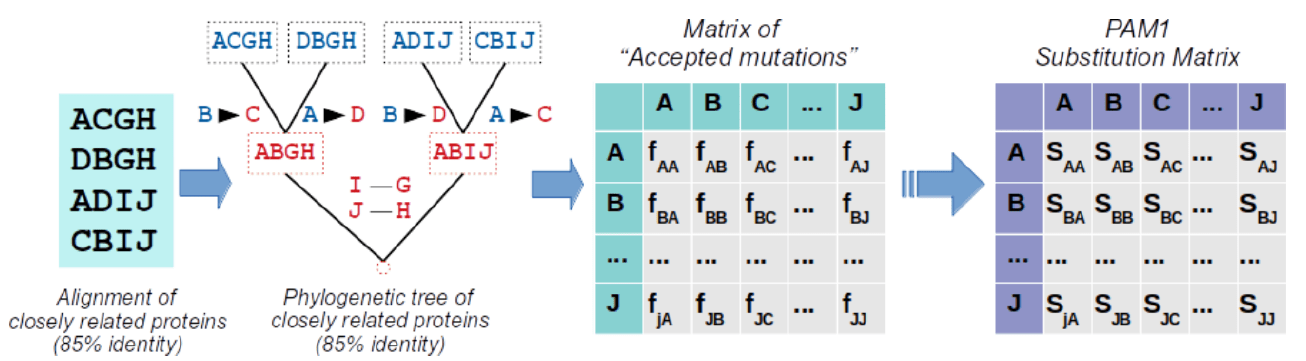
\includegraphics[width = \textwidth]{figs/pam-matrix.png}
\caption{\textbf{Generación de la matriz de sustitución PAM1.} A partir de alineaciones de secuencias estrechamente relacionadas (> 85\% de identidad), Margaret Dayhoff y sus colegas derivaron el árbol filogénico que representaba la evolución de la familia que requería el menor número de mutaciones. A partir de estos árboles contaron el número de veces que cada residuo fue sustituido por cualquier otro y registraron los valores en la matriz de mutaciones aceptadas. Por último, a partir de los datos de esta matriz generaron la matriz de sustitución PAM1 que representa la relación entre la probabilidad de la sustitución observada en el modelo evolutivo (suponiendo homología) y la probabilidad en el modelo aleatorio.}
\label{fig:pam}
\end{figure}

%04/10 - Luis del Peso
\subsubsection{Matrices de sustitución BLOSUM}
Más recientemente, el matrimonio Henikoff utilizó una familia de proteínas más alejada para poder inferir la frecuencia de sustitución en una matriz BLOSUM.

Para evitar la incertidumbre en los alineamientos, Dayhoff utilizó un conjunto de secuencias extremadamente relacionadas para derivar la PAM1. Sin embargo, las matrices PAM para proteínas más distantes se extrapolaron a partir de PAM1 en lugar de derivarse de la observación directa de los alineamientos reales. La acumulación de secuencias de proteínas en bases de datos a lo largo de los años permitió a Henikoff y Henikoff desarrollar un nuevo conjunto de matrices de sustitución a principios de los 90. Estas matrices, denominadas BLOCKS \footnote{un BLOCK se define como una región no superpuesta en el alineamiento de secuencias múltiples de menos de sesenta residuos de aminoácidos} amino acid SUbstitution Matrices (BLOSUM), se generaron al registrar cada posible sustitución de aminoácidos observada en los alineamientos de bloques. Utilizando alineamientos de proteínas que mostraban diferentes porcentajes de identidad, derivaron matrices BLOSUM que representaban la tasa de sustitución observada para diferentes grados de divergencia (figura \ref{fig:blosum}). Para ello, eliminan del bloque todas las secuencias que son idénticas en más de un x\% de posiciones, dejando una única secuencia representativa (por ejemplo, en BLOSUM62 se eliminaron las secuencias que compartían un 62\% de identidad o más). 

\begin{figure}[htbp]
\centering
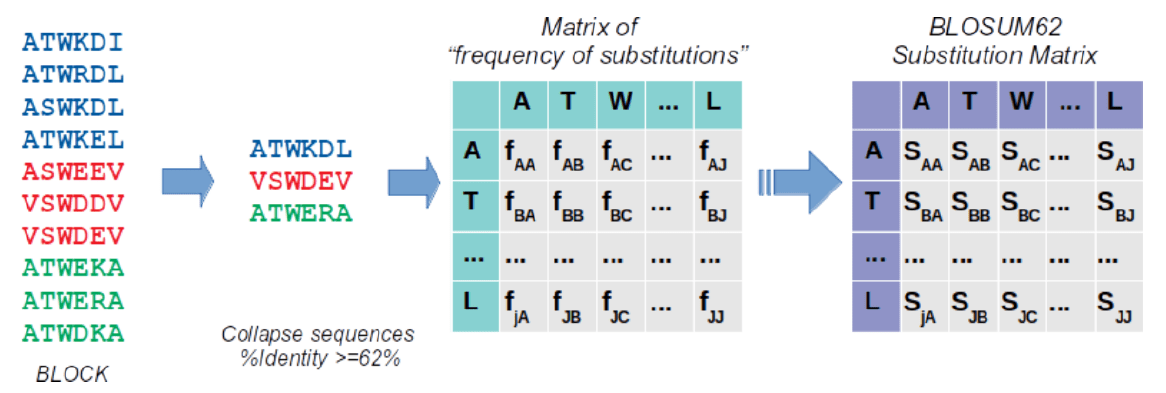
\includegraphics[width = \textwidth]{figs/blosum-matrix.png}
\caption{\textbf{Generación de la matriz de sustitución BLOSUM.} Partiendo de alineaciones sin colapsar de familias de proteínas (BLOCKS), Henikoff y Henikoff derivaron alineaciones que representaban diferentes distancias evolutivas colapsando todas las secuencias del bloque que compartían un umbral, C, de identidad. En la figura C = 62\%, todas las secuencias que comparten un porcentaje de identidad igual o superior al 62\% se muestran en el mismo color de fuente (primera columna), y luego se colapsan en un consenso que representa el clúster (segunda columna). A partir de estos alineamientos, contaron el número de veces que cada residuo i fue sustituido por cualquier otro y registraron los valores en la matriz de frecuencia de sustituciones. Por último, a partir de los datos de esta matriz generaron la matriz de sustituciones BLOSUM62 que representa la relación entre la probabilidad de la sustitución observada en el modelo evolutivo (suponiendo homología) y la probabilidad en el modelo aleatorio.}
\label{fig:blosum}
\end{figure}

Nótese que existen algunas diferencias importantes entre las matrices PAM y BLOSUM. En primer lugar, todas las matrices BLOSUM se derivan de la observación directa de alineamientos, mientras que sólo PAM se deriva de datos y el resto son extrapolaciones. En segundo lugar, mientras que PAM1 se generó a partir de alineaciones de secuencias estrechamente relacionadas (85\% de identidad), las matrices BLOSUM derivan de alineaciones que (pueden) incluir secuencias con un bajo porcentaje de identidad. Por último, para la construcción de PAM se infirieron sustituciones a partir de árboles filogenéticos derivados de los alineamientos. En BLOSUM no se construyó ningún árbol filogenético y las sustituciones se contaron a partir de la observación directa de los residuos alineados. Sin embargo, no se trata de sustituciones reales porque las secuencias alineadas evolucionaron a partir de un ancestro común y entre sí.

\subsubsection{Construcción de matrices de sustitución}
En las secciones anteriores vimos dos estrategias diferentes para determinar la frecuencia de cambios a partir de la observación empírica de alineamientos de proteínas homólogas. Dejando a un lado los detalles, ambos métodos producen una \textbf{matriz de frecuencia de mutación} \footnote{la suma de todas las entradas de la matriz da 1}, donde las entradas $q_{a,b}$, representan la \textbf{probabilidad observada} de encontrar los residuos a y b \textbf{alineados en proteínas homólogas}. En otras palabras, $q_{a,b}$, corresponde al término $p(alineado|homólogo)$. Ahora, para obtener el valor de la entrada para los residuos a y b en la matriz de sustitución correspondiente, necesitamos calcular el término $p(alineado|aleatorio)$, que sería la \textbf{probabilidad esperada}. En el modelo aleatorio suponemos que las dos proteínas alineadas no están relacionadas y no existen restricciones estructurales o funcionales que puedan causar correlación entre los residuos en una posición dada. Así, en este modelo la probabilidad de encontrar los residuos a y b alineados sólo depende de su frecuencia en las proteínas. En el modelo aleatorio no existe correlación alguna entre los residuos alineados en una posición dada, por lo que la probabilidad de observar a en una secuencia y b en la otra son independientes de modo que:

$$p(alineado|aleatorio) = p(a \cap b) = p_a p_b $$

donde $p_a$, y $p_b$, son las frecuencias de a y b respectivamente. La probabilidad de observar a y b alineados en estos dos modelos puede compararse tomando el cociente de las probabilidades, denominado \textbf{odds ratio}: $q_{a,b}/(p_a p_b)$. Cuando la probabilidad en el modelo evolutivo es mayor que en el modelo aleatorio, el odds-ratio toma cualquier valor entre 1 e infinito. Sin embargo, cuando la probabilidad en el modelo aleatorio es mayor, la odds-ratio está entre 0 y 1. Para evitar esta asimetría, se suele tomar el logaritmo de la odds-ratio para obtener la \textbf{log-odds ratio}. Como veremos más adelante, tomar el logaritmo del odds-ratio también facilita el cálculo de la puntuación total de la alineación. Por lo tanto, la entrada en la matriz de sustitución correspondiente a a y b se calcula como:

$$ s_{a, b} = log \frac{q_{a, b}}{p_a p_b} = log \frac{p(cambio|modelo evolutivo)}{p(cambio|aleatorio)} = log \frac{p(observado)}{p(esperado)} $$

La figura \ref{fig:substitution} muestra las matrices de sustitución PAM250 y BLOSUM62. Dado que la puntuación del alineamiento a sobre b es la misma de b sobre a, estas matrices son simétricas. Por este motivo, normalmente sólo se representa la mitad de la matriz. Los números positivos significan que se han observado más veces el cambio de residuos que lo que cabría esperar por azar, por lo que debe haber alguna presión positiva para que se mantenga. En el caso de los números negativos, se debe a una selección negativa. Cuando es 0, el ratio es 1 y por tanto la frecuencia es la observada por azar, no hay ninguna presión. 

Un ejemplo: El triptófano tiene una frecuencia de mutación observada muy pequeña, pero en la tabla BLOSUM, su número es el más alto. Esto significa que es un aminoácido muy importante que no se puede cambiar por ningún otro. Así, la tabla de frecuencias per se no refleja el parecido entre residuos, ya que hay que tener en cuenta la frecuencia. Sin embargo, la tabla BLOSUM sí refleja el parecido entre los residuos.   

\begin{figure}[htbp]
\centering
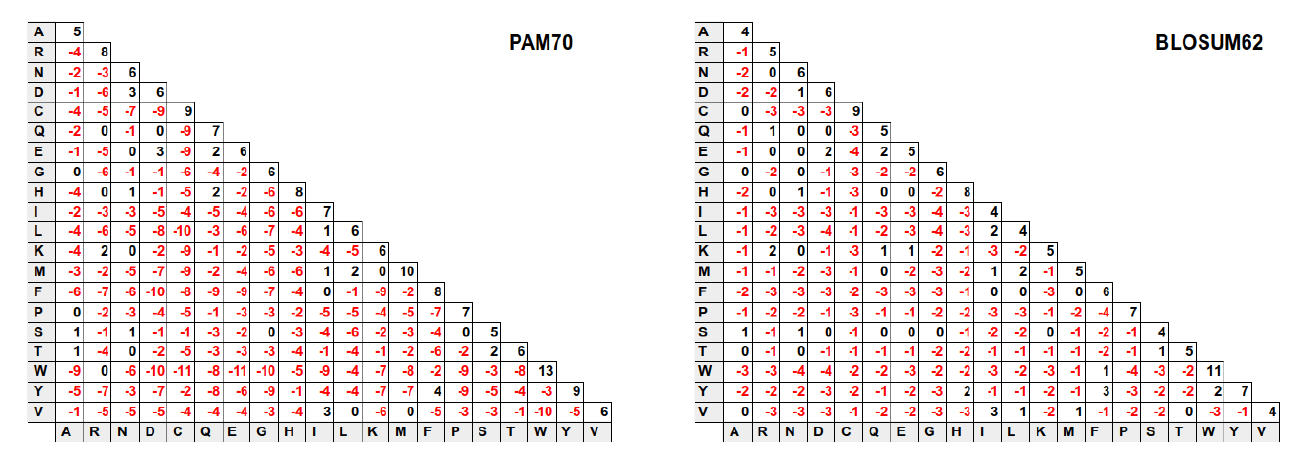
\includegraphics[width = \textwidth]{figs/substitution-matrix.png}
\caption{\textbf{Matrices de sustitución de aminoácidos.} La figura muestra las matrices de sustitución PAM250 (izquierda) y BLOSUM62 (derecha). Los valores negativos (en rojo) indican las sustituciones que tienen más probabilidades de observarse en el modelo aleatorio que en el evolutivo.}
\label{fig:substitution}
\end{figure}

\begin{table}[htbp]
\begin{mdframed}[backgroundcolor=black!10]
\textbf{Ejemplo de cálculo de matriz puntuación y odds ratio: Cambio D-L} \\
La matriz de frecuencia de mutación observada indica que el cambio D-L se ha observado 15 veces en 10000, es decir, 15/10000. La frecuencia de los bloques es 0,054 para D y 0,099 para L. Esto representa la frecuencia esperada. La puntuación se calcularía siguiendo la fórmula:

$$s = 2 \cdot \log_2(odds ratio) = 2 \cdot \log_2(\frac{observado}{esperado})$$

Sustituyendo los valores:

$$s = 2 \cdot \log_2(\frac{15/10000}{0,054 \cdot 0,099}) = -3,66 \approx -4$$

Cuando hay números decimales, se redondea al siguiente número entero. Al comprobar el valor en la matriz BLOSUM, el resultado efectivamente es -4.
\end{mdframed}
\end{table}

%\begin{figure}[htbp]
%\centering
%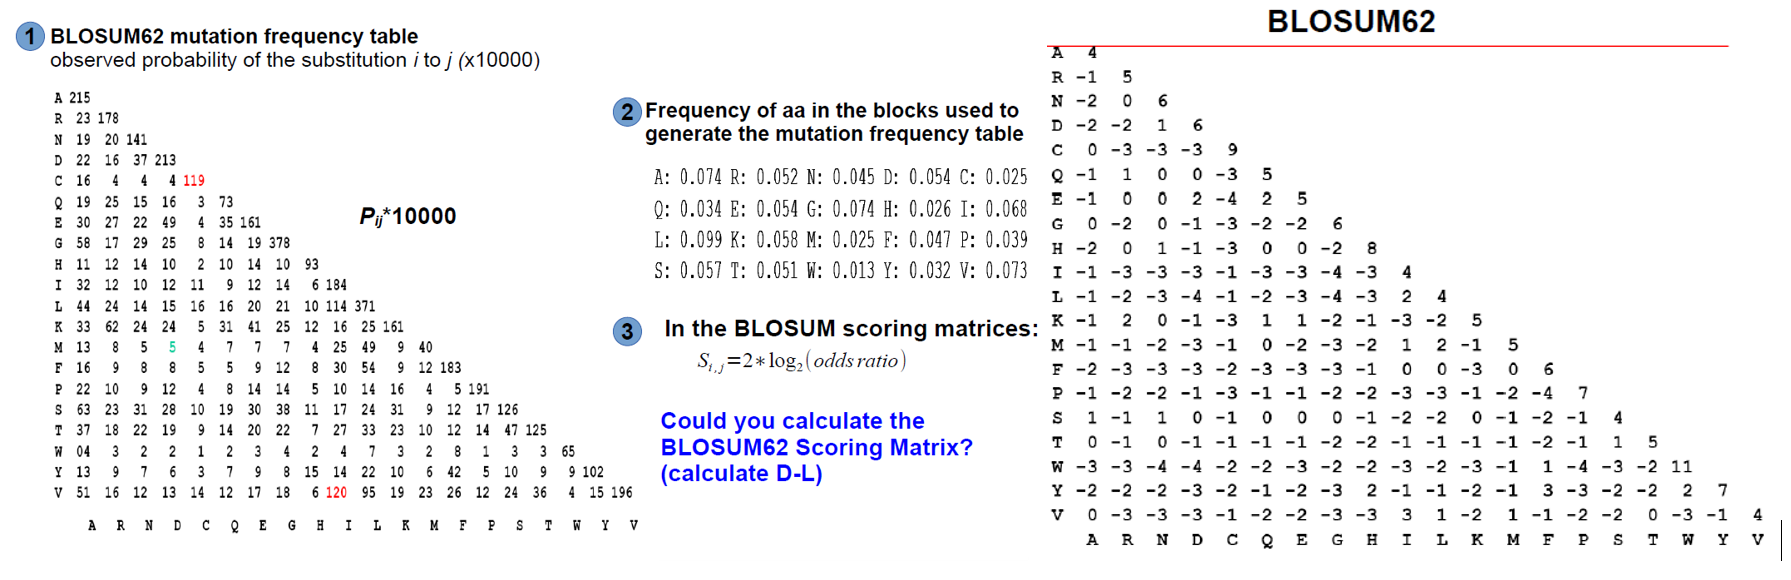
\includegraphics[width = \textwidth]{figs/ejercicio-blosum.png}
%\end{figure}

\subsubsection{Ejercicio}
\textit{\textbf{Ejercicio 1:} Queremos hacer una matriz de puntuación de ADN a partir de alineaciones de secuencias de ADN que muestren un 88\% de identidad (es decir, una matriz optimizada para encontrar alineaciones con un 88\% de identidad). Supongamos que todos los desajustes son equiprobables, y que la composición tanto de los alineamientos como de las secuencias de fondo es uniforme al 25\% para cada nucleótido. Construya la matriz de probabilidad de mutación y la matriz de puntuación. Introduzca los valores para la Matriz de Probabilidad de Mutación.}

Sabemos que las secuencias muestran un 88\% de identidad. Por tanto, en un 88\% de las ocasiones, las dos secuencias tienen los mismos residuos en la misma posición. Como cada nucleótido es equiprobable, $0,88/4 = 0,22$. Eso nos deja con $1 - 0,88 = 0,12$ a repartir entre los mismatches. Hay 12 posibilidades (12 casillas), y como todos son equiprobables, $0,12 / 12 = 0,01$. Ahora queda rellenar la tabla:

\begin{table}[htbp]
    \centering
    \begin{tabularx}{\textwidth}{ X | X X X X}
          & A & C & G & T \\ \hline
         A & 0,22 & 0,01 & 0,01 & 0,01 \\
         C & 0,01 & 0,22& 0,01 & 0,01 \\
         G & 0,01 & 0,01 & 0,22 & 0,01 \\
         T & 0,01 & 0,01 & 0,01 & 0,22 \\
    \end{tabularx}
\end{table}

En cuanto a la matriz de puntuación, nos indican que:
$$score = log_2(odds-ratio) = log_2(\frac{observado}{esperado})$$

El valor observado es aquel que obtenemos de la matriz de sustitución. El valor esperado es la probabilidad de los nucleótidos en ambas secuencias. Como una posición tendrá dos residuos (uno de cada secuencia), y todos los residuos son equiprobables, el valor esperado en cada caso será de $0,25 \cdot 0,25 = 0,0625$. Por ejemplo:

$$p_{AA} = log_2(\frac{0,22}{0,0625}) = 1,8 \approx 2$$
$$p_{AC} = log_2(\frac{0,01}{0,0625}) = -2,64 \approx -3$$

Así, la tabla resultante sería:

\begin{table}[htbp]
    \centering
    \begin{tabularx}{\textwidth}{ X | X X X X}
          & A & C & G & T \\ \hline
         A & 2 & -3 & -3 & -3 \\
         C & -3 & 2& -3 & -3 \\
         G & -3 & -3 & 2 & -3 \\
         T & -3 & -3 & -3 & 2 \\
    \end{tabularx}
\end{table}

%07/10
\subsection{Alineamientos de puntuación (scoring alignments)}
Las matrices de sustitución ofrecen un método para puntuar posiciones individuales. Sin embargo, para comparar diferentes alineaciones, necesitamos un único valor que represente la puntuación combinada de todas las posiciones. Para calcular dicha puntuación, suponemos que cada posición del alineamiento es independiente de las demás \footnote{Nótese que esto es probablemente una simplificación excesiva porque en las proteínas reales a menudo existe una correlación entre residuos adyacentes. Por ejemplo, en una hélice anfipática los residuos polares e hidrófobos se distribuyen en caras opuestas. Por lo tanto, habrá cierta correlación entre los residuos en ciertas posiciones.} y calculamos la puntuación del alineamiento S como la suma de las puntuaciones individuales de cada una de las n posiciones, siendo s la entrada de la matriz de sustitución para los residuos a y b en la posición i.

$$S = \sum_{i = 1}^{n} (s_{a,b})_i$$

En otras palabras, se pueden sumar los valores de las matrices BLOSUM de cada posición al haber utilizado el logaritmo. Ahora, esta función de puntuación sólo funciona para coincidencias y discordancias pero no tiene en cuenta los INDELs. Para representar los INDEL, un residuo o una serie de residuos en una secuencia de la alineación se empareja con guiones («-») en la otra secuencia. Durante la puntuación, la presencia de un hueco en el alineamiento da lugar a una penalización por hueco que se resta de la puntuación total. Hay dos razones para penalizar los huecos. En primer lugar, un hueco implica una diferencia entre las secuencias comparadas y, por tanto, reduce nuestra certeza sobre su origen común. Los huecos corresponden a eventos de inserción/deleción que ocurrieron durante la evolución desde el ancestro común en uno de los linajes. Por lo tanto, en general, cuanto mayor sea el número de huecos, mayor será la distancia evolutiva entre las secuencias. La segunda razón es que, introduciendo un número ridículo de huecos, podríamos aumentar artificialmente el número de coincidencias y, como consecuencia, aumentar la puntuación del alineamiento, aunque el alineamiento resultante no tendría sentido desde el punto de vista biológico. Así, las penalizaciones por huecos actúan limitando la introducción de huecos. Por lo general, el usuario establece la penalización por hueco a partir de un conjunto de valores predefinidos \footnote{En algunos programas, la penalización por hueco varía en función del tipo de residuo con el que se alinea el hueco. La razón es que algunos residuos tienden a estar fuertemente conservados debido a su impacto en la estructura/función. Por lo tanto, es más probable que la supresión de esos residuos altere la estructura/función y, por lo tanto, sufra selección negativa.} que se han determinado empíricamente a partir de la observación de su efecto en los alineamientos.

Otro aspecto a considerar es la longitud del hueco. Una forma de abordarlo es el esquema de \textbf{puntuación lineal de huecos}. Si $\delta$ es la penalización por la inserción o eliminación de un único símbolo, entonces $\kappa \delta$ sería la penalización por un hueco de longitud $\kappa$. Sin embargo, este modelo de costes implica que $\kappa$ huecos independientes tienen la misma penalización que un único hueco de longitud $\kappa$, lo que es inadecuado desde una perspectiva evolutiva. Los INDEL son el resultado de errores durante la replicación o reparación del ADN que provocan la limitación de un tramo de nucleótidos. Por tanto, una brecha, independientemente de su longitud, suele derivarse de un único evento de mutación, mientras que las brechas independientes surgieron por diferentes eventos de mutación.

En consecuencia, los \textbf{modelos de puntuación de huecos afines} diferencian la penalización por hueco abierto, la penalización aplicada la presencia de cada hueco independiente, y la penalización por extensión del hueco, que es menor que la anterior y es lineal con la longitud del hueco. La penalización por hueco afín se calcula a partir de estas dos penalizaciones diferentes como:

$$\delta + (\epsilon \cdot \kappa)$$

donde $\delta$ es la penalización por hueco abierto, $\epsilon$ la penalización por hueco extendido y $\kappa$ la longitud del hueco \footnote{Dependiendo del esquema de puntuación, $\kappa$ es la longitud del gap o la longitud del gap menos 1.} (número de residuos eliminados/insertados, es decir, guiones en la alineación). La penalización por hueco afín es el modelo de puntuación más popular. Impone una penalización mayor a los huecos más grandes. Aunque una brecha grande implica obviamente más diferencias a nivel de secuencia que una brecha más pequeña, ambas se produjeron como consecuencia de un único evento de mutación. Por este motivo, también se ha desarrollado una \textbf{puntuación constante de las diferencias}, que aplica una penalización a toda la diferencia, independientemente de su longitud.

Ahora podemos incorporar la penalización por hueco a la puntuación de alineación. La puntuación total del alineamiento se sigue calculando como la suma de las puntuaciones parciales en cada posición, de modo que para las coincidencias o discordancias utilizamos el valor $s_{a,b}$ de la matriz de sustitución y en los casos en que el símbolo de una de las secuencias sea un guión aplicamos la penalización por hueco. Definimos $\sigma_{a,b}$ como la función

$$\sigma (a, b) = \begin{cases}
s_{a,b} & \text{cuando} a \wedge b \neq gap \\
GapPenalty & \text{cuando} a \vee b = gap
\end{cases} $$

Y la puntuación del alineamiento como:

$$S = \sum_{i = 1}^{n} (\sigma(a,b))_i$$

\begin{table}[htbp]
\begin{mdframed}[backgroundcolor=black!10]
En resumen, hay consenso que, cuantos más gaps hay, más penalización debe recibir. Sin embargo, no hay consenso en cuanto a la penalización de los gaps, y hay tres esquemas:
\begin{itemize}
\item \underline{Gap penalty constante}: solo se tiene en cuenta si se ha abierto un gap, independientemente de su longitud.
\item \underline{Gap penalty linear}: se tiene en cuenta la extensión o longitud del gap.
\item \underline{Gap penalty afín}: Se tiene en cuenta si se ha abierto un gap y su longitud. Este esquema es el que se suele utilizar.
\end{itemize}

De esa forma, si los residuos a y b son, en un alineamiento, diferentes a "-" (es decir, no son gaps), se utiliza la matriz de sustitución. Si a o b son un gap, se emplea el gap penalty. 
\end{mdframed}
\end{table}

\begin{figure}
\centering
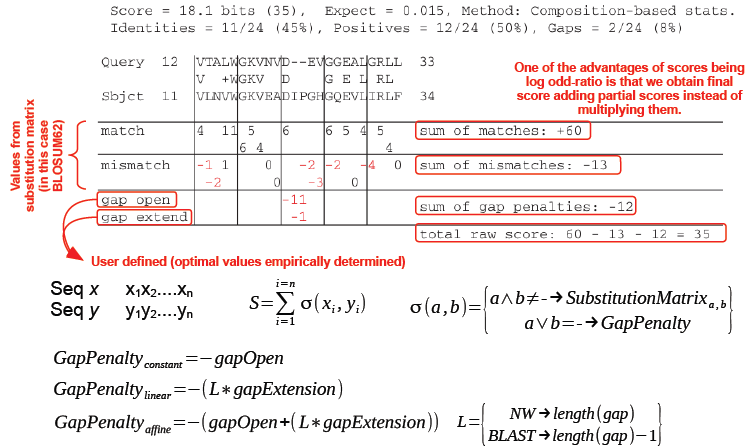
\includegraphics[width = \textwidth]{figs/gap-penalty.png}
\caption{Ejemplo de alineamiento con matriz de sustitución. Se han separado los valores de match y mismatch simplemente porque no cabían todos en línea. Los valores de penalización de apertura y extensión de gap los define el usuario de forma empírica. La longitud del gap se calcula de forma distinta en el algoritmo de Needleman-Wunsch que en BLAST.}
\end{figure}

\subsubsection{Ejercicio}
Calcula la puntuación del siguiente alineamiento: \\
TCCGGGGATCCCC-AGCA 17\\
TC--GGGATCCCCCATCA 16\\ 
Utilizando la siguiente matriz de puntuación:

\begin{table}[htbp]
    \centering
    \begin{tabularx}{\textwidth}{ X X X X X}
          & A & C & G & T \\ \hline
         A & +1 & -4 & -4 & -4 \\
         C & -4 & +1 & -4 & -4 \\
         G & -4 & -4 & +1 & -4 \\
         T & -4 & -4 & -4 & +1 \\
    \end{tabularx}
\end{table}

y penalización de gap de acuerdo con la expresión $G+L \cdot n$, donde G y L son las penalizaciones de existencia y extensión respectivamente y n la longitud del gap. En este caso, considera que la existencia (G) es 5 y la extensión (L) es 2. 

En este caso, la puntuación del alineamiento sería de:
$$+1 +1 -(5 +2 \cdot 2) +1 +1 +1 +1 +1 +1 +1 +1 +1 -(5 +2 \cdot 1) +1 -4 +1 +1 = -6$$

\subsection{Algoritmos de alineamiento}
Una vez que tengamos un método de puntuación, podríamos encontrar la alineación óptima entre dos proteínas enumerando todas las alineaciones posibles y eligiendo la de mejor puntuación. Sin embargo, este \textbf{enfoque de fuerza bruta} es poco práctico en términos de tiempo. El número de alineaciones posibles para dos secuencias de longitud m y n es $m^n$. Esto significa que un ordenador tiene que hacer un número de cálculos proporcional a $m^n$ para encontrar el alineamiento óptimo utilizando este enfoque de fuerza bruta. Así, pueden producirse más de $10^209$ alineaciones diferentes entre dos proteínas de tamaño medio (unos 350 residuos). Incluso procesando varios miles de alineaciones por segundo, el proceso duraría más que la edad del universo utilizando los ordenadores actuales. Afortunadamente, los bioinformáticos han encontrado formas inteligentes de reducir el tiempo de cálculo necesario para encontrar el mejor alineamiento posible, como se explica en las secciones siguientes.

\subsubsection{Algoritmos, complejidad del tiempo y notación de la big-O}
Un algoritmo puede definirse vagamente como un conjunto de pasos que pueden seguirse para alcanzar un objetivo. El conjunto de reglas que aprendiste en la escuela para multiplicar dos números largos es un ejemplo de algoritmo. El algoritmo define los pasos necesarios en un nivel abstracto; para que un ordenador siga los pasos, el algoritmo debe implementarse en un programa informático concreto. Así, un programa es la implementación de un algoritmo diseñado para realizar una tarea específica. En informática, la complejidad temporal describe el tiempo que se tarda en ejecutar un algoritmo. Dado que la velocidad de los distintos ordenadores varía, la complejidad temporal suele estimarse contando el número de pasos elementales que realiza el algoritmo, en lugar de en tiempo real. 

Los informáticos utilizan la notación big-O para describir de forma concisa el tiempo de ejecución de un algoritmo. En concreto, describe cómo crece el tiempo necesario para realizar el cálculo en función del tamaño de la entrada. 

\begin{figure}[htbp]
\centering
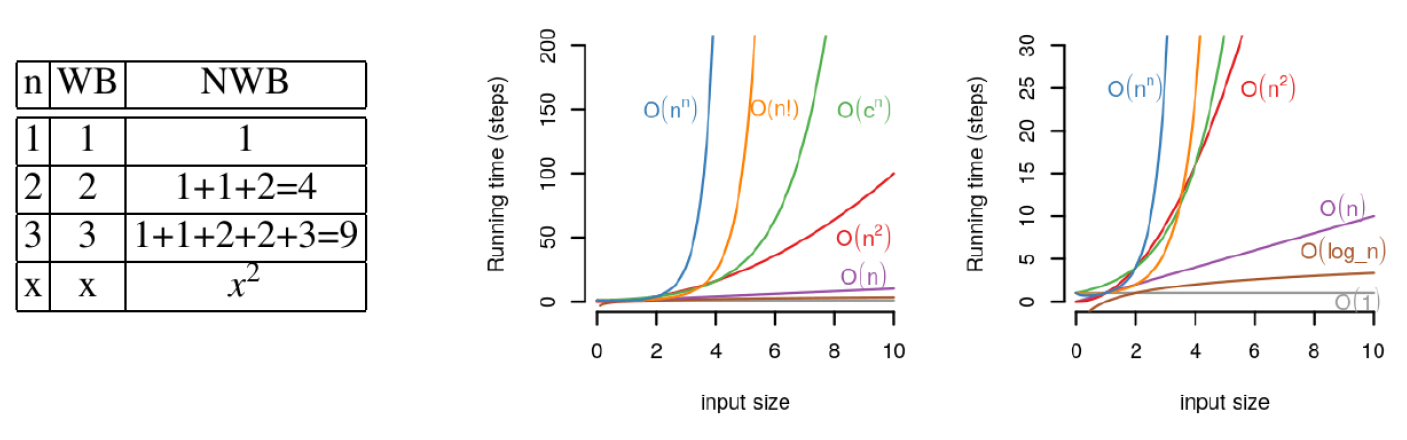
\includegraphics[width = \textwidth]{figs/big-o.png}
\caption{\textbf{Complejidad del tiempo y notación O grande}. La tabla a la izquierda de la figura muestra la comparación de los tiempos de carrera con y sin carretilla. El número de pasos que el trabajador debe caminar para construir una cerca de la longitud indicada ((n)) utilizando los algoritmos “carretilla” ((WB)) y “no carretilla” ((NWB)). Los gráficos de la derecha muestran la comparación de los tiempos de ejecución de algoritmos con diferentes complejidades temporales. Cada gráfico representa el número de pasos (eje y, "tiempo de ejecución") en función del tamaño de la entrada (eje x) para algoritmos con la complejidad de tiempo indicada: O(1), tiempo constante; O(log(n)), tiempo logarítmico; O(n), tiempo lineal; O($n^2$), tiempo cuadrático; O($c^n$) donde c es una constante, tiempo factorial; O(n!), tiempo factorial; O($n^n$), tiempo. Ambos gráficos son idénticos excepto por el valor máximo del eje y.}
\label{fig:big-O}
\end{figure}

Un ejemplo de juguete puede ser útil para comprender estos conceptos. Imaginemos que un trabajador construye una valla con ladrillos grandes. Si el trabajador utiliza una carretilla para transportar los ladrillos, el número de pasos (pasos físicos) que debe dar para construir la valla sería proporcional a la longitud de la valla. En este caso decimos que el «algoritmo» para construir la valla tiene una complejidad temporal lineal. Esto significa que si para una valla de 10 m de longitud el trabajador debe caminar un total de x pasos, para una valla de 50 m debe caminar 5x pasos. Imagina ahora que el trabajador no tiene carretilla. En este caso, debe coger el primer ladrillo, caminar y pasos para colocarlo y, a continuación, retroceder y pasos hasta el origen para coger el segundo ladrillo. Para colocar el segundo ladrillo, camina 2y para colocarlo más 2y pasos de vuelta al origen para coger el siguiente ladrillo, etc. La figura \ref{fig:big-O} compara el número de pasos de cada «algoritmo» en función del “tamaño de la entrada” que, en este ejemplo de juguete, es la longitud de la valla. El algoritmo «sin carretilla» muestra una complejidad temporal cuadrática, porque el número de pasos es proporcional al cuadrado del tamaño de la entrada. Usando la notación big O, «carretilla» es un algoritmo con complejidad temporal O(n), donde n es el tamaño de la entrada, mientras que «sin carretilla» es un algoritmo con complejidad temporal O($n^2$). Aunque ambos algoritmos darán el mismo resultado, «sin carretilla» tardará más que «carretilla» para cualquier longitud de valla (excepto n=1). Además, cuanto más larga sea la entrada (longitud de la valla a construir), mayor será la diferencia en pasos y, por tanto, en tiempo de ejecución (véase la figura \ref{fig:big-O}).

\subsubsection{Análisis de matriz de puntos (dot matrix alignment)}
Es el método más sencillo para comparar similitudes entre dos secuencias. Aunque es un método visual que no proporciona el alineamiento real, se utiliza a menudo para evaluar rápidamente, de un vistazo, la similitud entre dos secuencias. En este método, una de las secuencias se sitúa en el eje horizontal de una matriz con celdas vacías y la otra secuencia en el vertical. A continuación, cada uno de los residuos de una de las secuencias se compara con todos los residuos de la otra y se coloca un punto en la celda situada en la intersección de ambos residuos siempre que se produzca una coincidencia (residuo idéntico o similar en ambas secuencias). En esta representación, las regiones similares (tramos alineados de la secuencia) se muestran como diagonales en la matriz (véase la figura \ref{fig:dotplot}). El análisis de la matriz de puntos puede revelar fácilmente la presencia de inserciones/deleciones (huecos en la diagonal principal) y repeticiones directas/invertidas (diagonales paralelas/perpendiculares a la principal).

\begin{figure}[htbp]
\centering
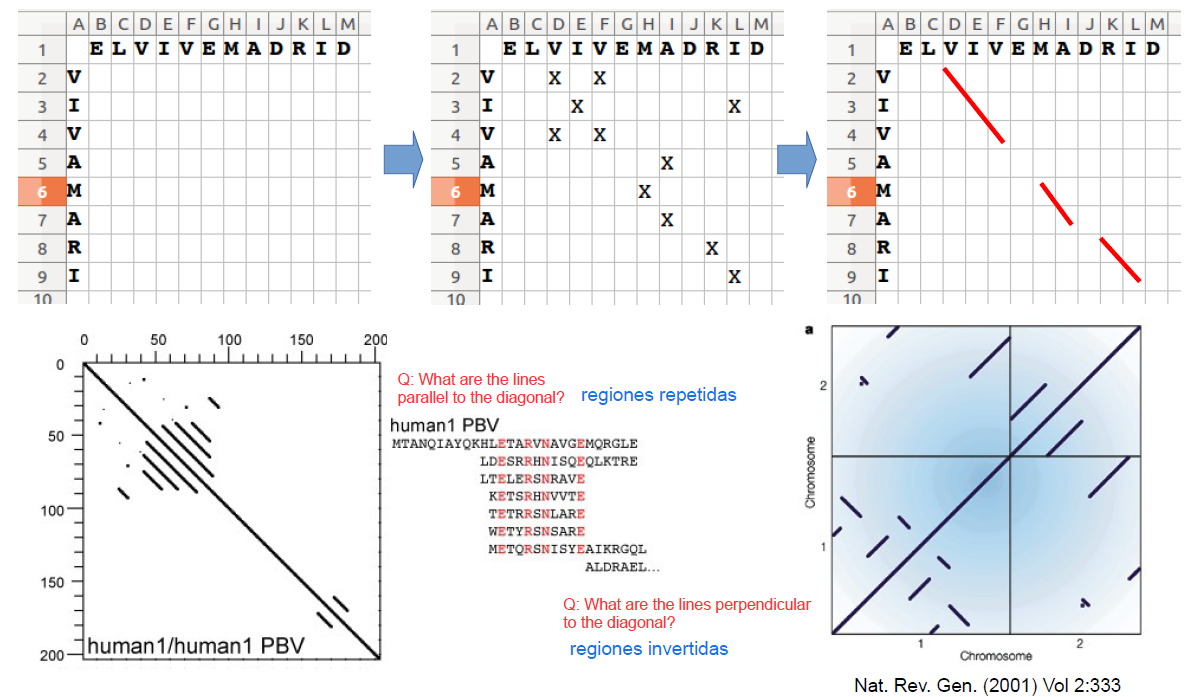
\includegraphics[width = \textwidth]{figs/dot-plot.png}
\caption{\textbf{Alineación matricial de puntos.} En su versión más sencilla, el análisis de matriz de puntos rellena una matriz de 2 dimensiones con coincidencias entre residuos de ambas secuencias y une las celdas diagonales adyacentes para producir el gráfico. La figura indica los pasos para producir el gráfico de izquierda a derecha. Las identidades se muestran en rojo oscuro y las similitudes en rojo claro.}
\label{fig:dotplot}
\end{figure}

\subsubsection{Programación dinámica}
Como ya se ha comentado, encontrar el mejor alineamiento posible mediante un algoritmo de fuerza bruta tiene una complejidad temporal de O($m^n$), lo que resulta poco práctico para alineamientos que impliquen más de unos pocos residuos. Afortunadamente, los algoritmos \textbf{Needleman-Wunsch} y \textbf{Smith- Waterman} son capaces de calcular el alineamiento óptimo entre dos proteínas en un tiempo muy ordenado. La diferencia entre ellos es que \textbf{Needleman-Wunsch calcula el alineamiento global} entre las proteínas, mientras que \textbf{Smith-Waterman produce alineamientos locales}. Los alineamientos globales contienen los residuos de las dos secuencias que se están alineando. Por el contrario, los alineamientos locales tratan de encontrar la región o regiones de mayor similitud entre las dos secuencias y producen un alineamiento (o varios) que contienen sólo los residuos incluidos en la región de alta similitud despreciando el resto de la secuencia. Los alineamientos locales son importantes para identificar regiones de gran similitud entre secuencias que, de otro modo, no comparten mucha identidad. Dado que las proteínas son modulares, es decir, contienen diferentes dominios funcionales, el alineamiento local permite identificar dominios compartidos entre proteínas con diferentes arquitecturas de dominio (figura \ref{fig:global-local}). Por ejemplo, aunque existen muchas proteínas quinasas diferentes pertenecientes a distintas familias, todas ellas contienen un dominio quinasa. Sin embargo, este dominio suele estar combinado con otros dominios que son específicos de cada familia de quinasas. Las quinasas AKT contienen un dominio de homología Pleckstrine (PH), necesario para la unión de fosfoinositidos, que se encuentra N-terminal al dominio quinasa. En cambio, las proteínas cinasas dependientes de cGMP contienen dos regiones de unión a cGMP, pero no un dominio PH, N-terminal a su dominio cinasa. No tendría mucho sentido intentar un alineamiento global entre estas dos quinasas, pero un alineamiento local revelaría una fuerte región de similitud correspondiente al dominio quinasa. 

\begin{figure}[htbp]
\centering
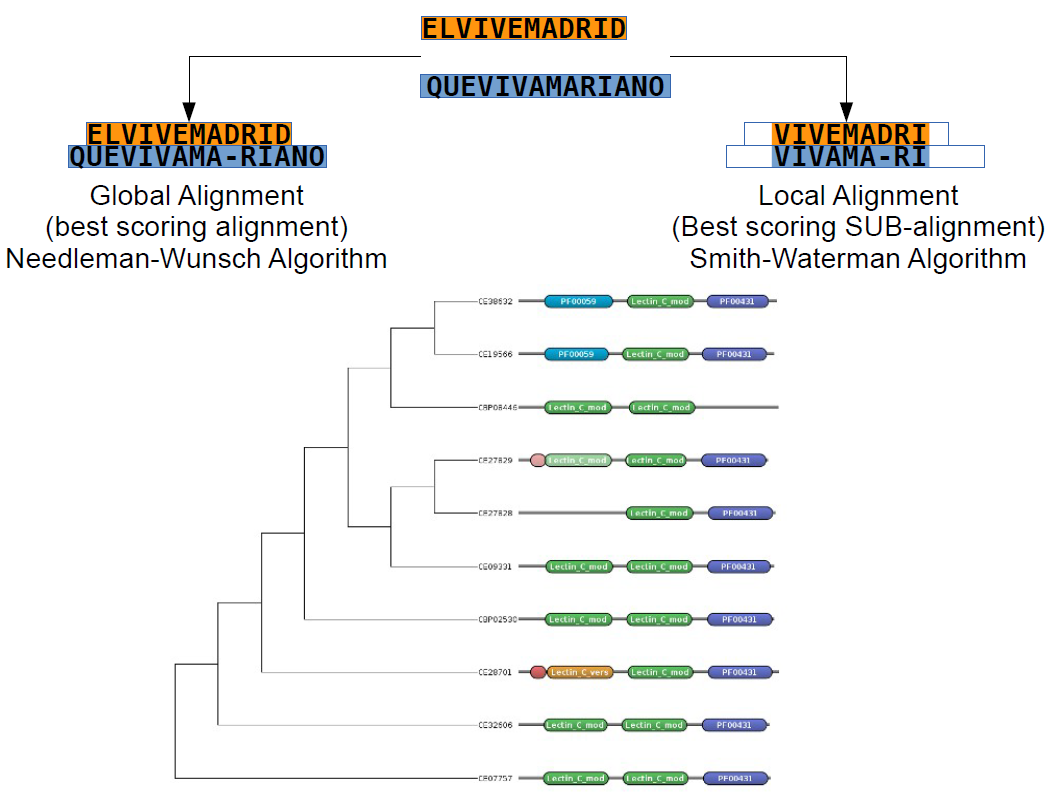
\includegraphics[width = 0.65\textwidth]{figs/alineamientos-global-local.png}
\caption{Comparación de un alineamiento global y local y su representación gráfica con los dominios de distintas proteínas.}
\label{fig:global-local}
\end{figure}

Ambos algoritmos, el de Needleman-Wunsch y el de Smith-Waterman, se basan en un método computacional llamado \textbf{programación dinámica}, que garantiza proporcionar el alineamiento óptimo (es decir, el mejor o el de mayor puntuación) para un par dado de secuencias en un tiempo proporcional a n $\cdot$ m (puesto que m $\approx$ n, entonces O($n^2$), es decir, tiempo cuadrático). Como se muestra en la figura \ref{fig:big-O}, estos algoritmos son mucho más rápidos, lo que permite calcular el alineamiento óptimo de forma práctica. Es importante destacar que los algoritmos de programación dinámica proporcionan la mejor alineación posible de acuerdo con un conjunto dado de reglas (puntuación por una coincidencia y penalizaciones por coincidencias erróneas y huecos), es decir, de acuerdo con un modelo matemático para la alineación de secuencias. Sin embargo, no se garantiza que el alineamiento óptimo resultante sea biológicamente relevante. Obsérvese que incluso para dos secuencias aleatorias el algoritmo informará de su mejor (aunque en este caso biológicamente irrelevante) alineación posible.

Al utilizar un algoritmo de programación dinámica, el número de comparaciones necesarias se reduce drásticamente. Además, al calcular todos los alineamientos posibles entre dos secuencias hay algunas operaciones (comparación entre residuos concretos) que se repiten una y otra vez. La programación dinámica mantiene un registro de todos esos cálculos en una tabla, por lo que evita la repetición, lo que supone un enorme ahorro de tiempo. En resumen, al calcular todos los alineamientos posibles, muchos subalineamientos se repiten muchas veces. La programación dinámica guarda el resultado de cada cálculo parcial para que, si se necesita más adelante, no haya que repetirlo. 

\begin{figure}[htbp]
\centering
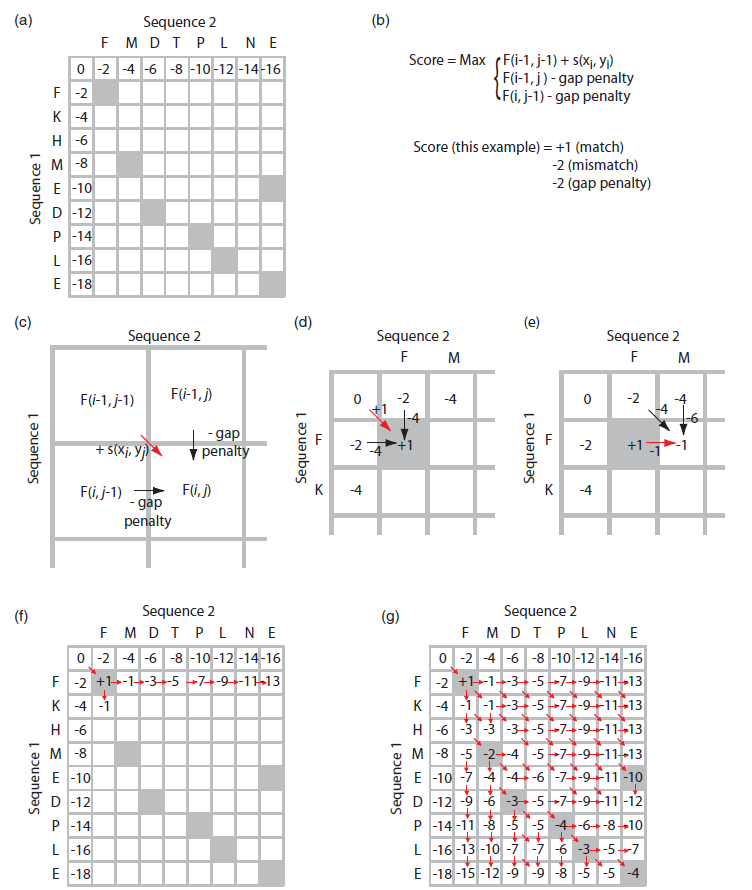
\includegraphics[width=0.8\textwidth]{figs/programacion-dinamica.png}
\caption{\small \textbf{Alineación por pares de dos secuencias de aminoácidos utilizando el algoritmo de programación dinámica de Needleman y Wunsch para el alineamiento global.} (a) Para secuencias de longitud m y n formamos una matriz de dimensiones m + 1 por n + 1 y añadimos penalizaciones por huecos en la primera fila y columna. Cada posición de hueco recibe una puntuación de -2. Las celdas que tienen identidad están sombreadas en gris. (b) El sistema de puntuación en este ejemplo es +1 para una coincidencia, -2 para una falta de coincidencia y -2 para una penalización por hueco. En cada celda, la puntuación se asigna utilizando el algoritmo recursivo que identifica la puntuación más alta a partir de tres cálculos. (c) En cada celda F(i, j) calculamos las puntuaciones derivadas de seguir un camino desde la celda superior izquierda (sumamos la puntuación de esa celda + la puntuación de F(i, j)), la celda de la izquierda (incluyendo una penalización por hueco) y la celda inmediatamente superior (de nuevo incluyendo una penalización por hueco). (d) Para calcular la puntuación de la celda de la segunda fila y columna, tomamos la máxima de las tres puntuaciones +1, -4, -4. Esta mejor puntuación (+1) sigue la trayectoria de la flecha roja, y mantenemos la información de la mejor trayectoria, resultante en la puntuación de cada celda para reconstruir posteriormente la alineación por pares. (e) Para calcular la puntuación de la segunda fila, tercera columna, volvemos a tomar el máximo de las tres puntuaciones -4, -1, -4. La mejor puntuación se obtiene a partir de la celda de la izquierda (flecha roja). (f) Procedemos a rellenar las puntuaciones de la primera fila de la matriz. (g) La matriz completada incluye la puntuación global del alineamiento óptimo (-4; véase la celda de abajo a la derecha, correspondiente al extremo carboxi de cada proteína). Las flechas rojas indican la(s) ruta(s) por la(s) que se obtuvo la puntuación más alta para cada celda.}
\label{fig:dynamic-programming}
\end{figure}

\normalsize
Para cada posición de un alineamiento, hay tres opciones posibles: que se alineen los residuos de ambas cadenas, que haya un gap en una cadena o que haya un gap en la otra cadena. La programación dinámica utiliza una matriz como la empleada en la figura \ref{fig:dynamic-programming}. Cuando se avanza de forma lateral (ya sea en horizontal o en vertical), se produce un gap en una u otra secuencia, mientras que cuando se avanza en diagonal, se produce el alineamiento de los dos residuos. Se rellena la matriz con las puntuaciones de cada uno de los movimientos y se marca aquel que sea más favorable. Si se produce alguna situación en la que haya dos valores máximos o iguales, es decir, dos direcciones que den el mismo score global, se escoge cualquiera de ellos ya que ambos alineamientos serían igual de buenos. El valor de la esquina inferior izquierda es el score global del alineamiento. Una vez rellena la matriz, se produce el alineamiento recorriendo el camino a la inversa siguiendo las direcciones más favorables. Un programa para calcular esto es \href{https://baba.sourceforge.net/}{BABA}, ya que permite introducir las secuencias, ajustar las penalizaciones por gaps e ir viendo cómo se rellena la matriz paso a paso. En este programa, las flechas están al revés, ya que indican de dónde vienen en lugar de a dónde van.

\begin{table}[htbp]
\begin{mdframed}[backgroundcolor=black!10]
\textbf{[Material adicional] Obtener el número de alineamientos posibles con gaps:} Las tres posibles formas de moverse en la matriz se puede resumir en dos vectores. El número de pasos que dar es la suma de los pasos que se dan desde el inicio al final del alineamiento. Sumando todos los caminos, se tendría el número de alineamientos posibles. El número de matches es igual al número de vectores (1,1). Para obtener el valor total, se utilizan los números combinatorios. Para calcular el número total global de todos los alineamientos, es el sumatorio de k (matches posibles) y el número mínimo de m y n.

$$\sum_{k=0}^{min(m,n)} = \begin{pmatrix}
          m + n - k \\
          k, m-k, n-k
    \end{pmatrix}$$
\end{mdframed}
\end{table}

\subsection{Relevancia estadística de la puntuación de alineamiento}
Los métodos de alineación devolverán la mejor coincidencia posible entre dos secuencias dadas. Sin embargo, es de vital importancia tener en cuenta que, dadas dos secuencias cualesquiera, los algoritmos de alineación siempre devolverán una alineación que sea la mejor posible según un conjunto de reglas matemáticas (el esquema de puntuación). Sin embargo, \textbf{ser el mejor posible no significa necesariamente que sea biológicamente relevante}. Por ejemplo, la proteína BAD (bcl2-associated agonist of cell death) es un miembro de la familia Bcl-2 y, como tal, un actor clave en el proceso de apoptosis, un tipo de muerte celular programada (PCD) bien caracterizado en animales. Aunque la PCD está documentada en plantas, la maquinaria responsable de impulsar el proceso sigue siendo esquiva y los reguladores apoptóticos, incluidos los miembros de la familia Bcl-2, aún no se han identificado en plantas. La figura \ref{fig:bad-thaliana} muestra la mejor coincidencia de la proteína BAD humana en la planta \textit{Arabidops thaliana}. Ahora bien, ¿es esta proteína putativa de \textit{A. thaliana} un verdadero homólogo de la proteína BAD humana o se trata simplemente de la mejor coincidencia posible según nuestro esquema de puntuación, aunque no tenga un ancestro común con BAD? 

\begin{figure}[htbp]
\centering
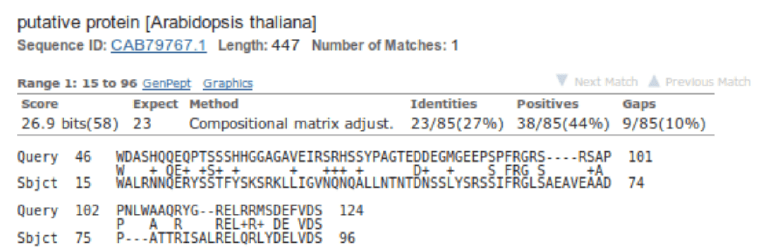
\includegraphics[width = \textwidth]{figs/bad-thaliana.png}
\caption{\textbf{¿Homólogo vegetal de BAD?} Alineación del mejor resultado de una búsqueda BLAST utilizando la proteína humana BAD (NP-004313.1) como consulta frente a las proteínas de \textit{Arabidopsis thaliana} (taxid:3702). El Expect se fijó en 100 y el resto de parámetros BLAST se dejaron con los valores por defecto.}
\label{fig:bad-thaliana}
\end{figure}

En el análisis de alineamientos de proteínas, la puntuación que se obtiene al comparar diferentes secuencias es clave para determinar la posible homología entre ellas (cuanto mayor sea la puntuación, mayor será la probabilidad de que las proteínas deriven de un ancestro común). Sin embargo, la mera comparación de puntuaciones no es suficiente para asegurar que las secuencias están relacionadas evolutivamente; es necesario un análisis estadístico más profundo para descartar que las similitudes observadas se deban al azar. En otras palabras, ¿cómo de grande debe ser la puntuación para que concluyamos que las proteínas son homólogas?
El concepto central es la \textbf{hipótesis nula}, que asume que el alineamiento observado es producto de secuencias no relacionadas (aleatorias). Para evaluar esta hipótesis, es necesario comparar la puntuación obtenida ($s_{ab}$) con la distribución de puntuaciones que se obtendrían al alinear proteínas no homólogas o generadas aleatoriamente. De esta manera, podemos calcular un \textbf{p-valor} empírico, que representa la probabilidad de obtener una puntuación igual o superior a la observada simplemente por azar. Este p-valor se calcula como la proporción de veces que un alineamiento aleatorio supera la puntuación observada, proporcionando una medida objetiva de la significancia del alineamiento.
Por otra parte, si la distribución de las puntuaciones aleatorias sigue una distribución estadística conocida (por ejemplo, una distribución normal), podemos aplicar las herramientas de la inferencia estadística para calcular el valor p exacto. Sea cual sea el método utilizado para calcular el valor p, empírico o exacto, indica la probabilidad de que la puntuación $s_{ab}$ se deba al azar. Podemos aceptar la alineación como significativa (posiblemente indicando homología) si su puntuación está en el 5\% superior (u otro valor elegido) de las puntuaciones generadas aleatoriamente (p <0,05).

Por ejemplo, al comparar las proteínas NP-508008 (proteína 1) y NP-29564 (proteína 2), el alineamiento obtuvo una puntuación de 55,5, mientras que al comparar NP-508008 con NP-001421 (proteína 3), el valor fue de 477. A pesar de que ambos alineamientos presentaban valores similares en identidad, similitud y gaps, las diferencias en las puntuaciones indican posibles diferencias evolutivas entre los pares de proteínas. Para evaluar la relevancia de estos scores, se realizó un alineamiento de la proteína 1 con una secuencia generada aleatoriamente, y los valores obtenidos fluctuaron entre 8,5 y 100. Dado que el valor 55,5 del alineamiento entre las proteínas 1 y 2 cae dentro de este rango, podemos inferir que la similitud observada podría deberse al azar y, por tanto, no hay evidencia clara de una relación evolutiva significativa entre ellas. Por otro lado, la puntuación de 477 para el alineamiento entre las proteínas 1 y 3 se encuentra fuera del rango de valores aleatorios, lo que sugiere una relación evolutiva significativa. El p-valor para el alineamiento de las proteínas 1 y 2 se calculó como 0,34 (34\%), lo que indica que el 34\% de los alineamientos aleatorios tienen puntuaciones iguales o superiores a 55,5. Dado que este valor es mayor que el umbral típico de significancia (p < 0,05), no se puede rechazar la hipótesis nula, lo que sugiere que la similitud observada es posiblemente un producto del azar. En cambio, en el caso del alineamiento entre las proteínas 1 y 3, no se observó ninguna puntuación aleatoria cercana a 477, lo que implica que la probabilidad de que esta similitud sea debida al azar es extremadamente baja. Por lo tanto, para concluir si dos secuencias están evolutivamente relacionadas no es suficiente con observar una alta puntuación en el alineamiento; es necesario calcular un valor estadístico como el p-valor que permita definir con precisión la relevancia de dicho alineamiento. En resumen, el algoritmo Needleman-Wunsch nos proporciona una herramienta para generar alineamientos óptimos, pero carece de la capacidad para distinguir si un alineamiento tiene o no base biológica, razón por la cual es crucial el uso de métodos estadísticos adicionales para interpretar correctamente los resultados.

%09/10 - Luis del Peso
\textbf{Ejercicio práctico (problema de programación):} Partiendo de un script que computa el alineamiento entre dos secuencias de aminoácidos, se debe modificarlo para calcular el p-valor empírico asociado al score del alineamiento.  Se deben dar dos secuencias de entrada, y se debe obtener un p-valor asociado al score como salida.

\subsection{Métodos basados en k-tuplas o palabras} %Alineamiento heurístico: BLAST
El alineamiento por pares rara vez se utiliza para comparar dos secuencias dadas, sino que suele emplearse para buscar en una base de datos con una secuencia de consulta para identificar secuencias similares. A pesar de la eficacia de los algoritmos de alineación basados en la programación dinámica, el gran tamaño de las bases de datos actuales haría que las búsquedas con estos métodos exactos fueran demasiado lentas \footnote{En las bases de datos biológicas, a día de hoy se estima que hay $10^8$ - $10^9$ residuos, y una proteína normal tiene $10^2$ - $10^3$ residuos. Así, la matriz de scoring tendría que tener $10^3$ residuos en un lado y $10^8$ en el otro, por lo que el rastreo tarda horas.}. Por este motivo se desarrollaron nuevas alternativas más rápidas a los métodos de programación dinámica: FASTA y el muy popular BLAST (Basic Local Alignment Search Tool). Para aumentar la velocidad de la búsqueda, estos programas no realizan un alineamiento exacto (es decir, óptimo) entre la consulta y cada una de las secuencias de la base de datos, sino que estos métodos primero escanean la base de datos en busca de posibles coincidencias y luego realizan un alineamiento más preciso con ellas. Sin embargo, la mayor velocidad tiene un precio. A diferencia de los métodos dinámicos, no se garantiza que FASTA y BLAST encuentren los alineamientos óptimos. Los métodos o algoritmos que cambian precisión por velocidad se denominan heurísticos. Así, FASTA y BLAST son \textbf{algoritmos heurísticos} que permiten buscar en bases de datos mucho más rápido que los métodos precisos, como Needleman-Wunsch y Smith-Waterman, pero que no garantizan devolver el mejor alineamiento posible (óptimo). La estrategia utilizada por FAST y BLAST para reducir el tiempo de búsqueda consiste en dividir la consulta en k-mers \footnote{En bioinformática, los k-mers son subsecuencias de longitud k contenidas en una secuencia más larga.} o palabras e identificar secuencias en la base de datos que contengan coincidencias exactas (o casi exactas) con cualquiera de los k-mers de la consulta. A continuación, se puntúan las coincidencias en la base de datos y las mejores se amplían mediante programación dinámica.
Una búsqueda en la base de datos con el algoritmo BLAST sigue estos pasos:
\begin{enumerate}
\item Hace una lista de todas las palabras k-mers contenidas en la secuencia de consulta. La longitud de la palabra se fija por defecto en 3 residuos (3-mer) para las búsquedas de proteínas y en 11 residuos (11-mer) para los ácidos nucleicos. No obstante, el valor del parámetro del tamaño de la palabra (word size) puede ser modificado por el usuario para adaptar la búsqueda a necesidades específicas. Cuanto menor sea el word size, mayor será la sensibilidad, pero requiere más semillas que extender y un mayor tiempo de computación. 
\item Para cada una de las palabras derivadas de la consulta, el algoritmo identifica todas las palabras similares que, según la matriz de sustitución elegida, darían lugar a una puntuación superior a un umbral predefinido en un alineamiento por pares. El umbral se obtiene por BLAST de forma empírica. Las palabras resultantes son las palabras de alta puntuación, HSW (high scoring words).
\item El algoritmo busca en las secuencias de la base de datos coincidencias exactas con cualquiera de las HSW. Cada coincidencia, denominada High-scoring Segment Pair (HSP), se utiliza en el siguiente paso para ampliar este alineamiento semilla.
\item Cada HSP identificado en el paso anterior se extiende entonces en ambas direcciones hasta que la puntuación total del HSP creciente comienza a disminuir.
\item Todos los HSP con una puntuación superior a un umbral predefinido se retienen y el BLAST calcula el alineamiento local Smith-Waterman entre la consulta y la secuencia objetivo en el HSP.
\end{enumerate}

\begin{figure}[htbp]
\centering
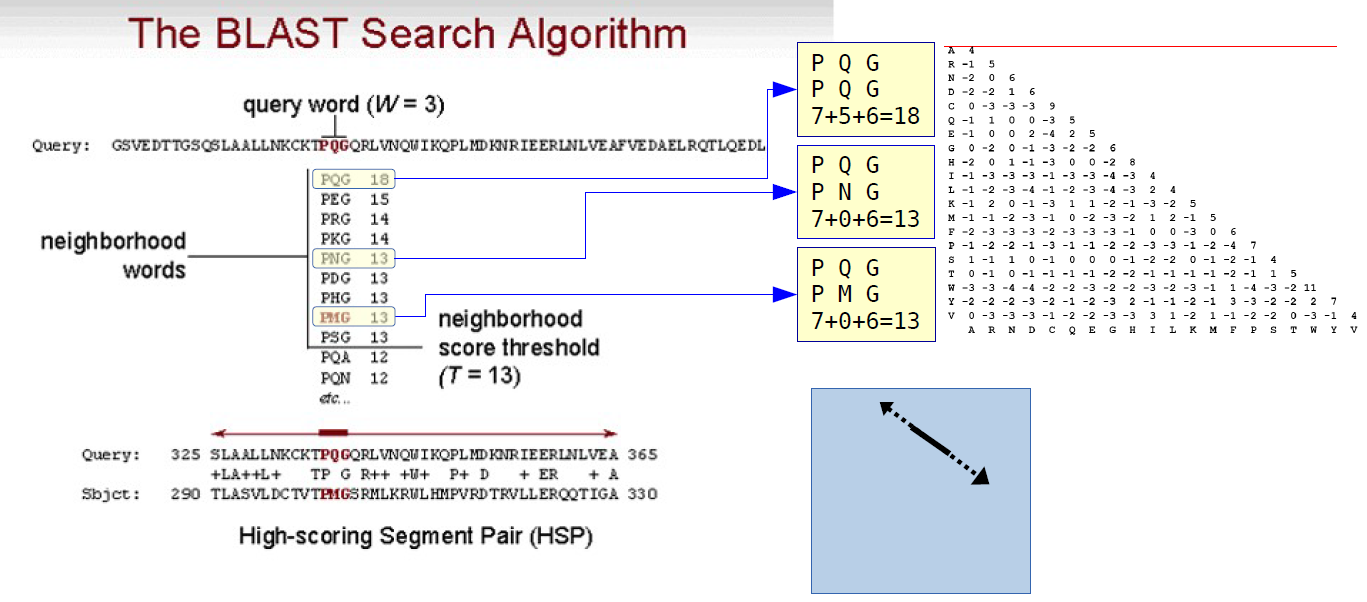
\includegraphics[width = \textwidth]{figs/blast-algorithm.png}
\caption{Ejemplo de una búsqueda mediante BLAST.}
\end{figure}

BLAST no informa de un valor p como tal, sino que proporciona el \textbf{valor E} o valor esperado (Expect value). BLAST se emplea normalmente para buscar en una base de datos con una consulta y el valor E es un parámetro que describe el número de resultados que uno puede "esperar" ver por casualidad al buscar en una base de datos de un tamaño determinado. Cuanto más bajo sea el valor E, más significativa será la puntuación y la alineación (se considera que un valor es significativo cuando el valor E es menor que $10^-4$). Además, el valor E disminuye si el tamaño de la base de datos disminuye (si solo se tiene cuenta una especie, por ejemplo). El valor E se relaciona con el valor p mediante la ecuación:
$$p = 1 - e^{-E}$$

El valor E en el alineamiento mostrado en la figura \ref{fig:bad-thaliana} es 23, lo que significa que se esperarían 23 alineamientos con una puntuación igual o mejor que 26,9 bits sólo por azar. Además, el valor p asociado es 1, por lo que no descartamos la hipótesis nula (la puntuación sí pertenece a la distribución aleatoria).

\subsection{Interpretación biológica de alineamientos de secuencia: identificación de secuencias afines}
Como ya hemos mencionado, uno de los usos más importantes del alineamiento de secuencias es la búsqueda en bases de datos con el objetivo de identificar secuencias relacionadas con una consulta. Se considera que las secuencias similares están conservadas evolutivamente, es decir, que derivan de un ancestro común y, por tanto, deberían tener una estructura/función similar. Sin embargo, una vez que tenemos un alineamiento, ¿cómo decidimos (basándonos en él) si las secuencias están relacionadas o no? En otras palabras, ¿cuán similares deben ser dos secuencias para ser consideradas homólogas? Evidentemente, cuanto mayor sea el porcentaje de residuos similares, mayor será la probabilidad de que sean homólogas. El límite inferior suele fijarse en el 25-30\% de identidad para las secuencias de aminoácidos y en más del 70\% para las de nucleótidos. Es importante señalar que esas recomendaciones se aplican a secuencias de más de 100 residuos, ya que es probable encontrar un alineamiento de alta puntuación con consultas de secuencias cortas. Por debajo de este umbral se encuentra una región, denominada \textbf{Twilight zone}, en la que no podemos estar seguros de que las similitudes encontradas sean relevantes. Desde una perspectiva estadística, la inspección de las identidades porcentuales tiene una utilidad limitada en la Twilight zone (identidad inferior al 25\%) porque no proporciona un conjunto riguroso de reglas para inferir homología, y se asocia con resultados falsos positivos o falsos negativos. En ocasiones, un alto grado de identidad en una región corta podría no ser evolutivamente significativo y, a la inversa, un bajo porcentaje de identidad podría reflejar homología. Así pues, el porcentaje de identidad por sí solo no basta para demostrar (ni para descartar) la homología. Hay dos factores de confusión que debemos tener en cuenta al utilizar el porcentaje de identidad para evaluar la homología. El primero es la \textbf{longitud de las secuencias alineadas}. No es lo mismo observar un 25\% de identidad sobre 150 residuos que sobre 10. El segundo es la \textbf{distancia evolutiva}, obviamente dos homólogos realmente distantes compartirán un porcentaje de identidad menor que dos homólogos cercanos. Así pues, el porcentaje de identidad en sí mismo no es un criterio suficientemente sólido para evaluar la homología. A pesar de ello, algunos investigadores han sugerido que si dos proteínas comparten un 25\% o más de identidad de aminoácidos en un intervalo de 150 o más aminoácidos, es probable que estén significativamente relacionadas, y si dos proteínas comparten un 20\% - 25\% de identidad en un tramo razonablemente largo (por ejemplo, de 70 a 100 residuos de aminoácidos), se encuentran en la Twilight zone. Sin embargo, es importante tener en cuenta que dos proteínas que no están relacionadas en absoluto suelen compartir entre un 10\% y un 20\% de identidad por casualidad cuando se alinean.

\begin{figure}
\centering
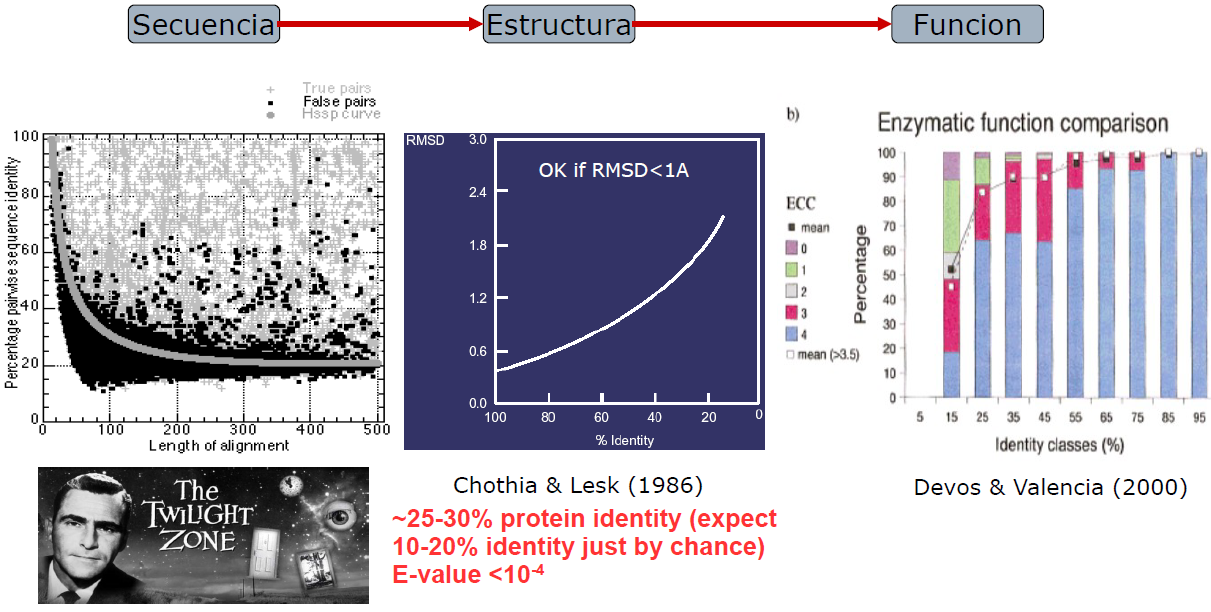
\includegraphics[width = \textwidth]{figs/twilight-zone.png}
\caption{Representaciones gráficas de la Twilight Zone.}
\end{figure}